\documentclass[11pt,a4paper]{article}

\usepackage[left=2cm,text={17cm,24cm},top=3cm]{geometry}
\usepackage[english]{babel}
\usepackage[utf8]{inputenc}
\usepackage[T1]{fontenc}

\usepackage{url}
\usepackage{float}
\usepackage{comment}
\usepackage{etoolbox}
\usepackage{graphicx}
\usepackage{hyperref}
\usepackage{tocloft}
\usepackage{pdfpages}
\usepackage{changepage}

\def\UrlBreaks{\do\/\do-\do\&\do=\do\_\do?} % URL breaking characters

\newcommand{\red}[1]{\textcolor{red}{#1}} % \red{text in red}
\newcommand{\blue}[1]{\textcolor{blue}{#1}} % \blue{text in blue}
\newcommand{\TODO}{\textbf{\textcolor{red}{TODO}}} % red bold TODO
\newcommand{\tilda}{\raisebox{0.5ex}{\texttildelow}} % command \tilda for '~' character

\graphicspath{{img/}} % path to images
\patchcmd{\thebibliography}{\section*{\refname}}{}{}{} % do not create section for bibliography
\hypersetup{
    linktoc    = all,
    colorlinks = true,
    citecolor  = green,
    linkcolor  = red,
    urlcolor   = blue,
}

\begin{document}

\begin{titlepage}

    \begin{center}
        % FIX: lines must end with '%', if not then it will result in an incorrect centering
        \vfill {%
            \Huge{%
                \textsc{%
                    Faculty of Informatics\\[3mm]%
                    Masaryk University%
                }%
            }%
        }%

        \hfill\\[15mm]

        \begin{figure}[!h]
            \centering
            
\includegraphics[scale=3]{muni-fi-logo.pdf}
        \end{figure}

        \hfill\\[10mm]

        \Huge{
            \textbf{
                PV207
            }
        }

        \hfill\\[-10mm]

        \huge{
            \textbf{
                Business Process Management
            }
        }

        \hfill\\[10mm]

        \LARGE{
            \textbf{
                Homework (4th seminar)
            }
        }
        \vfill

    \end{center}

        \Large{
            \noindent Adrián Tóth (491322)\hfill \today
        }

\end{titlepage}

\setlength{\parskip}{0pt}
    {
        \hypersetup{
            hidelinks=true
        }
        \tableofcontents
    }
\setlength{\parskip}{0pt}

\newpage

\section{Informations}

\begin{center}
    \begin{tabular}{l|l}
        UČO           & 491322        \\
        Student Name  & Adrián Tóth   \\
        Seminar Group & PV207/01CZECH \\
    \end{tabular}
\end{center}

\section{Brief Summary}

    \subsection{Description}

        \begin{adjustwidth}{2.5cm}{2.5cm}

            \noindent A person (customer) walks into a hostel. The customer wishes to be accommodated (book a room) in place at the reception.\\

            \noindent There is a receptionist (hostel worker) in the hostel who can book a room for a customer in place via an information system.\\

            \noindent There is a need to select the desired room from a list of available (free) rooms by the customer. After room selection, it is necessary to collect information about the customer for the payment and the bill creation. After that, the payment is made, which must be verified. In the case of successfully processed steps before, the system books the room and creates a bill, which is passed to the customer by the receptionist.\\

            \noindent The capacity for all rooms is one. The necessary data and payment for the booking are required to be collected and verified before the room booking is made.\\

            \noindent We do not assume that it will be required to book a room for more than one person. The hostel is used just for one night by lonely persons.
        \end{adjustwidth}

\newpage

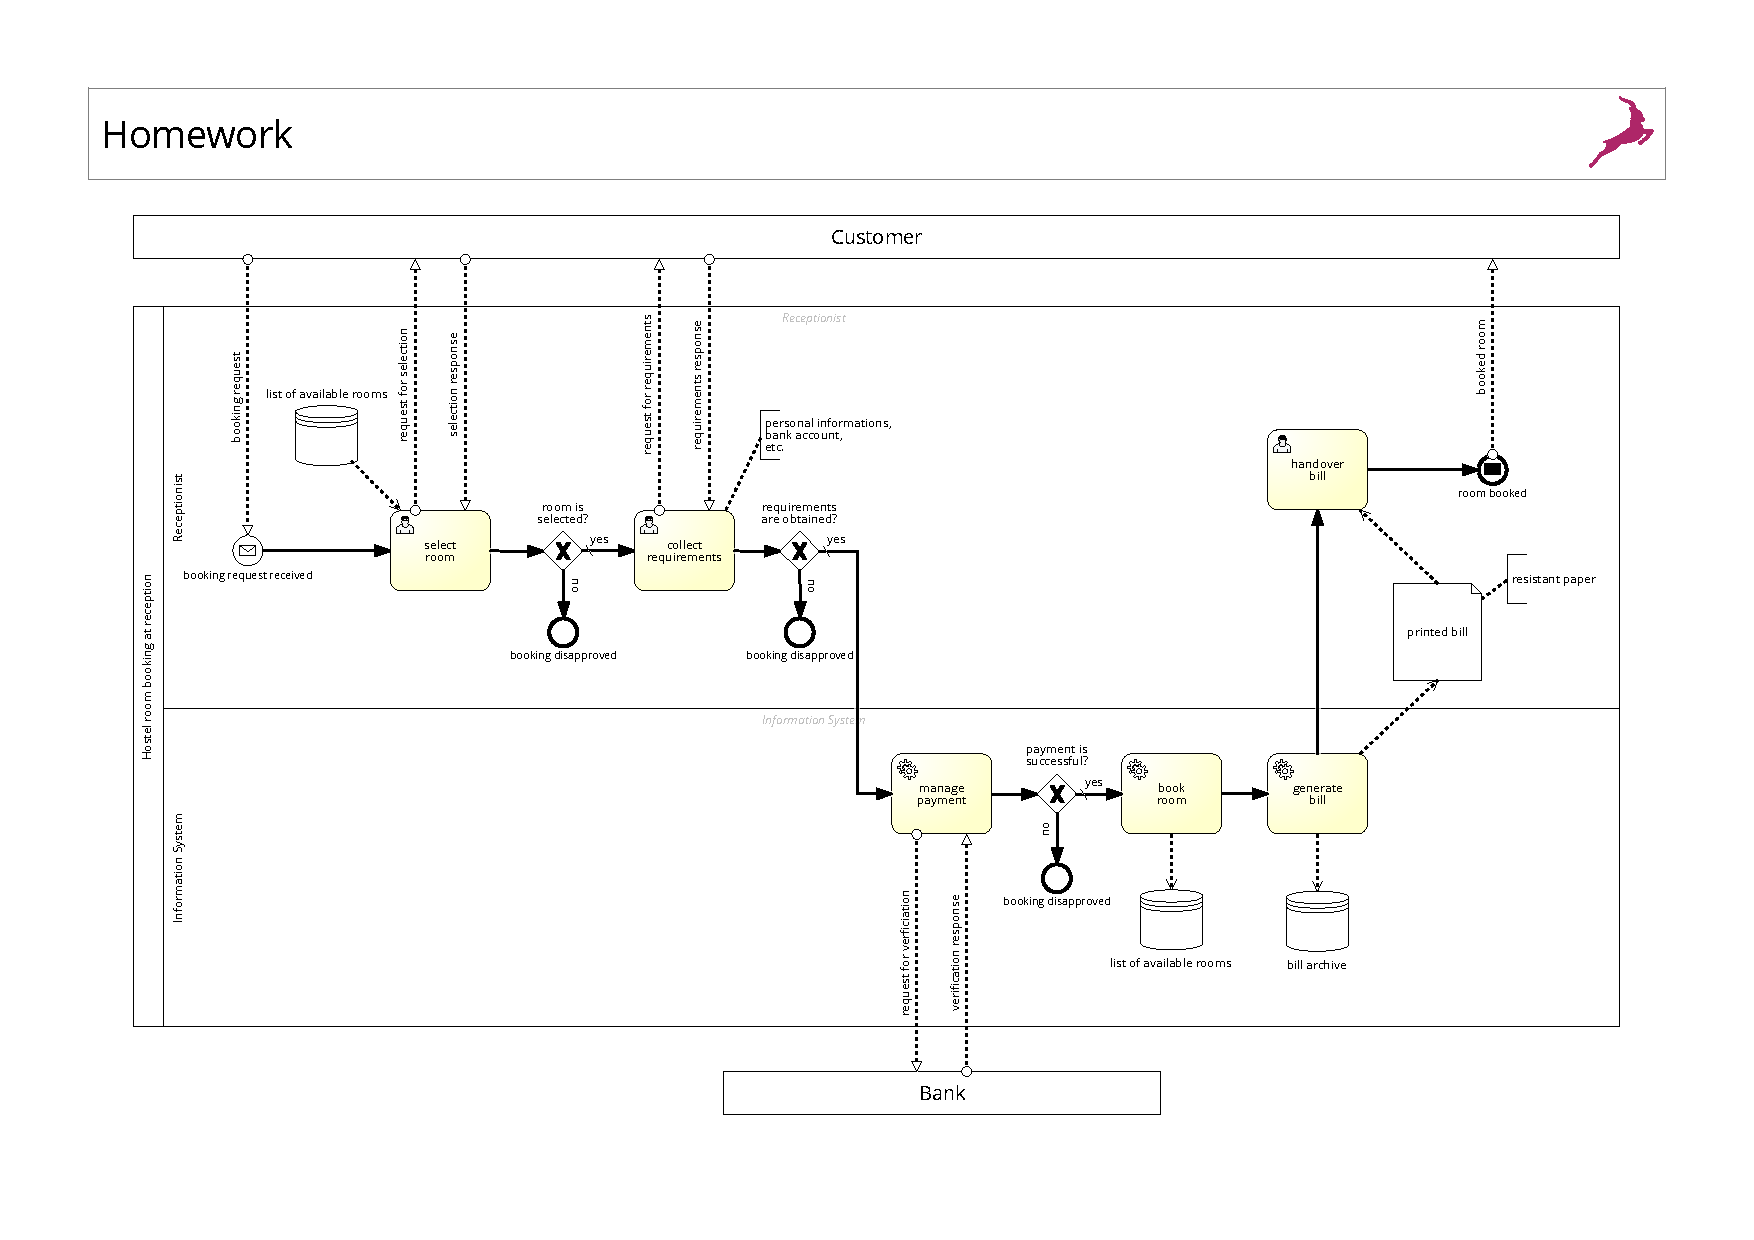
\includepdf[landscape=true]{Homework.pdf}

\end{document}
